\documentclass[conference]{IEEEtran}
\usepackage{cite}
\usepackage{amsmath,amssymb,amsfonts}
\usepackage{algorithmic}
\usepackage{graphicx}
\usepackage{textcomp}
\usepackage{xcolor}
\def\BibTeX{{\rm B\kern-.05em{\sc i\kern-.025em b}\kern-.08em
    T\kern-.1667em\lower.7ex\hbox{E}\kern-.125emX}}
    
\graphicspath{{./images/}}
\begin{document}

\title{Hybrid Recommender System Using Switching}

\author{\IEEEauthorblockN{Benjamin Russell, fdmw97}
\IEEEauthorblockA{\textit{Department of Computer Science} \\
\textit{Durham University}\\
Durham, United Kingdom}
}
\maketitle

\section{Introduction}
\subsection{Domain of Application}
The hybrid recommender system presented in this paper operates in the domain of recommending bars. More specifically the domain includes explicit ratings of said bars. As this domain is a form of hospitality venue similar methods can be used as with other such venues e.g. restaurants\cite{b1}.
\subsection{Related Work Review}
Personalised recommender systems are designed to predict a rating value for a user-item combination, based on training data in the form of user preferences for said items\cite{b2}. A hybrid recommender system builds on this by using multiple recommender systems to produce either a more accurate rating or to address the shortcomings of an individual recommender system\cite{b3}. Most commonly this hybrid is designed using a colloborative filtering based recommender with another recommender to try and avoid the cold-start problem\cite{b4}. The cold-start problem is the problem of recommending items to new users with few ratings or a new item with few ratings\cite{b5}, with both problems being present for collaborative filtering and the latter being lessened in content-based methods if a suitable item representation exists\cite{b4}. Research, in the form of an extensive literature review has shown that the most popular choice of algorithms for hybrid recommender systems is a collaborative and content based hybrid due to the aforementioned cold-start problem\cite{b5}. \par Within the chosen application domain there are multiple hybridisation methods available. The \textit{EntreeC} recommender system\cite{b1} used a cascade model where recommendations were first generated using a knowledge-based model and then further refined using a collaborative model. The recommender presented in\cite{b7} uses a switching hybrid that uses a collaborative filtering recommender if a user has left a sufficient number of reviews and a knowledge based recommender otherwise (in order to address the cold-start problem).
\subsection{Aim}
The rest of this paper aims to introduce a new hybrid recommender system called \textit{Bars4U}. This system will recommend an existing user a list of five bars to visit based on their previous reviews. Explainability of reviews is of the utmost importance in this system as is transparency to the user, therefore the interface for displaying the reviews must be clear and not obfuscate any important information. Addressing the cold-start problem is also paramount and therefore will inform the choice of hybridisation technique and the individual recommender system algorithms.


\section{Methods}
\subsection{Data Description}
The \textit{Yelp Open Dataset}\cite{b9} was used for \textit{Bars4U}. It consists of seven \texttt{.json} files, four of which were used during the development of \textit{Bars4U}. These files were \texttt{business.json, review.json, user.json, }and \texttt{covid.json} which contain information on businesses, reviews, users, and updated business information due to COVID-19 respectively. The data-set contains 8,021,122 reviews (ratings) and 209,393 businesses (items) meaning it is of considerable size and requires preprocessing before use. Businesses with fewer than 3 reviews were also omitted from the data-set.
\par The \texttt{user.json} file contains the user ratings in the form of an explicit rating ($1-5$ stars) and a textual review.
\subsection{Data Preparation and Feature Selection}
The large size of the data-set meant that using it all would be impractical due to memory constraints. Therefore businesses were removed from the \texttt{business.json} file that were not in the chosen domain of bars\textemdash the result was then stored in a \texttt{.csv} file. The 8,021,122 reviews in the data-set were then restricted to reviews relevant to the selected businesses and to a fixed 6 month time period, 2018-07-1--2018-12-31. Users that had not interacted with this set of businesses, during this 6 month period, were removed from the \texttt{user.json} file. Users and businesses that had few reviews were kept in the data-set as this would artificially reduce the effect of the cold-start problem rather than the hyrbid scheme reducing it instead. The COVID-19 data from \texttt{covid.json} was also restricted to only bars as well.
\par
All features from the businesses were used from the data-set, \texttt{attributes} and \texttt{categories} were used to represent each business as an item vector representation. \texttt{Attributes} consists of a series of nested objects that represent various properties the business has e.g. how loud it is. \texttt{Categories} is a list of strings describing what kind of business it is e.g. a karaoke bar. The remaining features were used by the recommender when presenting the recommendations to the user. Features about business location were not used when generating the recommendations as that was not within the scope of hybrid scheme used.
\par
The features extracted from the review data were a list of \texttt{user\_id} and each corresponding rating (\texttt{stars}), on the scale $1-5$. The textual review data (\texttt{review}) could have been used by performing semantic or textual analysis\cite{b10}. However this was not done due to the availability of the explicit ratings in the data-set and the possibility of introducing errors during the semantic analysis\cite{b11}.
\par
Very few features from the user data (\texttt{user.json}) were used, the \texttt{name} feature was used only for the interface and \texttt{review\_count} was used when determining switching criteria in the hybrid scheme.
\subsection{Hybrid Scheme}
\textit{Bars4U} uses a switching hybrid scheme. Switching hybrid recommenders use 2 or more separate recommender systems and choose which system to use for a prediction based on some criteria\cite{b2}. This was chosen as the hybrid scheme as analysis of the data-set showed that $26\%$ of businesses in the domain have fewer than 10 ratings, this is a clear example of the cold-start problem for new items\cite{b2}, a situation that switching recommenders were originally designed to address\cite{b4}. To this end \textit{Bars4U} uses a switching hybrid consisting of a collaborative filtering recommender, and a secondary content-based filtering recommender that is used in the case of an item having fewer ratings than a certain threshold.
\subsection{Recommendation Techniques}
The collaborative filtering component of \textit{Bars4U} uses the Single Value Decomposition method (SVD), this method is a form of matrix factorisation and is a model based approach to collaborative filtering rather than memory based\cite{b2}. This method is appropriate for this domain and data-set due to the size of it, even when stored as a sparse matrix the size of the similarity matrices for K-Nearest neighbour (KNN) collaborative filtering was prohibitive. A comparison of both KNN and SVD showed a marginally better accuracy for SVD as well.
\par
The content-based filtering component of \textit{Bars4U} uses the vector space model (VSM)\cite{b12}. This method uses a corpus (the set of items) and a dictionary (keywords related to the items), in the case of \textit{Bars4U} this method was appropriate due to the feature selection used. Since, for each business, the \texttt{attributes} and \texttt{categories} features were used, and these consist of words related to the business is makes sense to treat them as the dictionary. User profiles are stored as classifiers that use Rocchio's Method in order to predict a users rating\cite{b13}.
\subsection{Evaluation Methods}
Offline evaluation was used on \textit{Bars4U} in order to determine its performance. A different metric was used to measure accuracy of ratings, accuracy of usage predictions, coverage, and explainability respectively.
\par
Rating accuracy was measured using Root Mean Squared Error (RMSE) as defined by the following equation:
\begin{equation}
    RMSE=\sqrt{\frac{1}{\lvert\hat{R}\rvert}\sum_{\hat{r}_{ui}\in\hat{R}}(r_{ui}-\hat{r}_{ui})^{2}}
\end{equation}
where $\hat{R}$ is the set of predicted ratings and $r$ is the actual rating. RMSE was chosen due to it giving a high weight to large errors due to the squared term. This is desirable as a large error could give the user a much worse experience than a smaller one.
\par
Accuracy of usage predictions was measured using the precision metric:
\begin{equation}
    precision=\frac{TP}{TP+FP}
\end{equation}
where TP and FP are true and false positives respectively. This was chosen in order to measure how many of the recommendations are actually useful, as it would be poor to recommend one very useful prediction with 9 terrible ones.
\par
Coverage was measured using Catalog Coverage defined as:
\begin{equation}
    Catalog\ coverage=
    \frac
    {\lvert\bigcup_{j=1}^{N}I_{L}^{j}\rvert}
    {\lvert I \rvert}
\end{equation}
where $I$ is the set of all items and $I_{L}^{j}$ is the set of items recommended to user $j$.
\par
Explainability was measured using the Mean Explainability Precision (MEP)\cite{b14} defined by:
\begin{equation}
    \frac{1}{N}
    \sum_{j=1}^{N}
    \frac{\lvert I_{E}^{j}\rvert}{\lvert I^{j}\rvert}
\end{equation}
where $I_{E}^{j}$ is the set of explainable recommendations to user $j$ and $I_{j}$ is the set of recommendations to user $j$
\section{Implementation}
\subsection{Input Interface}
The interface for \textit{Bars4U} is a very simple command line interface. The active user is recognised by inputting the \texttt{user\_id} from a list of available IDs in \texttt{README.txt}. The user data is then gathered explicitly in the form of their reviews and \texttt{name}. Finally the user can either request a list of 5 recommendations or can update a rating for an item which then triggers the system to regenerate their user profile.
\subsection{Recommendation Algorithm}
From the main database of reviews and businesses a pivot table is generated as a matrix of \texttt{user\_id}, \texttt{business\_id}, and \texttt{stars}. This pivot matrix is then used with the SVD algorithm in which the predicted rating $\hat{r}_{ui}$ is given by:
\begin{equation}
    \hat{r}_{ui}=\mu+b_{i}+b_{u}+q_{i}^{T}p_{u}
\end{equation}
The SVD model is fit using the pivot table to learn the parameters $\mu$, $b_{i}$, and $b_{u}$ for later use.
\par
For each unrated item for the user, the \texttt{review\_count} feature is checked against the switching threshold value of 50 reviews (this value was chosen after testing showed it had the best balance of RMSE and runtime). If \texttt{review\_count} is greater than 50 then the item prediction is calculated using the fitted SVD model. If not then the content-based recommender is used. This model uses the \texttt{categories} and \texttt{attributes} features are collated into a bag-of-words for each rated item. The bag-of-words for all items are then converted into tf-idf vectors, resulting in a matrix of rated item vectors for the user. These vectors are then used to train a Rocchio Classifier (Nearest Centroid, using Euclidean distance as similarity measure), this classifier is then used to predict ratings for items with fewer than 51 ratings.
\subsection{Output Interface}
The output interface is designed for a computer monitor, and displays a list of 5 recommended bars in order of preference. The user can then enter the number of a bar to see more information about. This information is derived from the information in the pruned \texttt{business.json} file and includes things such as the location and opening times. At the bottom of the business information the predicted star rating is displayed to the user along with an explanation as to how this rating was predicted.
\section{Evaluation Results}
\begin{figure}[h]
    \centering
    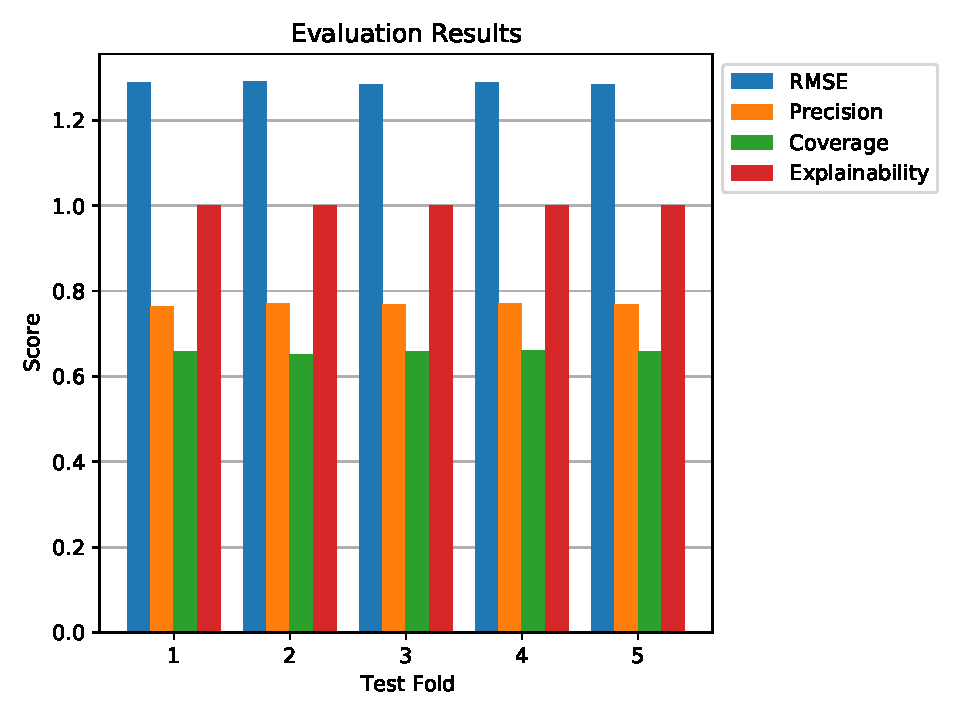
\includegraphics[width=0.3\textwidth]{result_graph}
    \caption{Evaluation metrics across 5 KFolds}
    \label{fig:res}
\end{figure}
RMSE has a mean value of $1.2871$ and a negligible standard deviation. This is an improvement on the baseline (SVD only) models RMSE of $1.3108$, although small this does show that the hybrid scheme did manage to improve accuracy by addressing the cold-start problem. Precision had an average of $0.7684$ compared to the baseline of $0.7667$, once again this shows a small increase over the baseline. Coverage had an average of $0.6571$ compared with $0.6542$ for the baseline, again a small increase for the hybrid. Explainability had a value of $1$, this was likely due to the choice of metric not taking confidence of recommendation into account, so all recommendations had an explanation. The baseline had an explainability of $0$ as it did not provide explanations.
\par
The hybrid recommender presented in\cite{b15} exhibited an RMSE of 0.8962 and precision of 0.7809. Both these results beat \textit{Bars4U} especially the RMSE. This is likely down to the collaborative filtering method used was SVD++ rather than SVD which has been shown to outperform SVD due to implicit ratings\cite{b15}.
\par
Two ethical issues were identified with \textit{Bars4U}. Due to the use of collaborative filtering being prioritised in the hybrid scheme bars that have many ratings will be recommended more than bars with fewer ratings, this could have a negative affect on businesses that are new or infrequently visited, as even if they are appropriate for a user, clearly this could harm these businesses. The location data of the bars could also potentially be used to de-anonymise users as it is likely they will have more ratings for bars located near to them, this could be addressed by encrypting the bar and user data when it is stored and not in use.
\section{Conclusion}
Although the switching hybrid scheme addresses the cold-start problem for items it does not solve it for users, this is particularly bad as the data-set has many users with as few as 1 review in it. In the future this could be addressed by using a method such as Feature-Augmentation\cite{b1} to generate placeholder reviews for users to be used in the collaborative filtering component of the recommender. The bars in the data-set are also located across multiple states in the \textbf{USA} this means some recommendations may be infeasible to travel to for users. This could be addressed by adding some sort of Case-based reasoning component\cite{b2} to the recommender as this would allow users to explicitly ask to recommendations only located near them or even with specific attributes they would like. Currently there is also nothing in place to allow the user to give feedback on the generated recommendations, this could be implemented in the future to generate a more accurate user profile in the form of a Knowledge based recommender\cite{b3}

\begin{thebibliography}{00}
\bibitem{b1}Burke, Robin \& Robin,. (2007). Hybrid Web Recommender Systems. LNCS. 4321. 10.1007/978-3-540-72079-9\_12.
\bibitem{b2}C. Aggarwal, Recommender Systems. Cham: Springer International Publishing, 2016, p. 3.
\bibitem{b3}E. Çano and M. Morisio, "Hybrid recommender systems: A systematic literature review", Intelligent Data Analysis, vol. 21, no. 6, pp. 1487-1524, 2017. Available: 10.3233/ida-163209
\bibitem{b4}R. Burke, User Modeling and User-Adapted Interaction, vol. 12, no. 4, pp. 331-370, 2002. Available: 10.1023/a:1021240730564
\bibitem{b5}B. Lika, K. Kolomvatsos and S. Hadjiefthymiades, "Facing the cold start problem in recommender systems", Expert Systems with Applications, vol. 41, no. 4, pp. 2065-2073, 2014. Available: 10.1016/j.eswa.2013.09.005
\bibitem{b7}P. Dwivedi and N. Chheda, "A Hybrid Restaurant Recommender", International Journal of Computer Applications, vol. 55, no. 16, pp. 20-25, 2012. Available: 10.5120/8840-3071
\bibitem{b9}"Yelp Dataset", Yelp.com, 2021. [Online]. Available: https://www.yelp.com/dataset.
\bibitem{b10}L. Chen, G. Chen and F. Wang, "Recommender systems based on user reviews: the state of the art", User Modeling and User-Adapted Interaction, vol. 25, no. 2, pp. 99-154, 2015. Available: 10.1007/s11257-015-9155-5
\bibitem{b11}D. Margaris, C. Vassilakis and D. Spiliotopoulos, "What makes a review a reliable rating in recommender systems?", Information Processing \& Management, vol. 57, no. 6, p. 102304, 2020. Available: 10.1016/j.ipm.2020.102304
\bibitem{b12}G. Salton, Automatic text processing. Reading, Massachusetts: Addison-Wesley, 1989.
\bibitem{b13}D. Tarragó, C. Cornelis, R. Bello and F. Herrera, "A multi-instance learning wrapper based on the Rocchio classifier for web index recommendation", Knowledge-Based Systems, vol. 59, pp. 173-181, 2014. Available: 10.1016/j.knosys.2014.01.008
\bibitem{b14}B. Abdollahi and O. Nasraoui, "Explainable Matrix Factorization for Collaborative Filtering", Proceedings of the 25th International Conference Companion on World Wide Web - WWW '16 Companion, 2016. Available: 10.1145/2872518.2889405
\bibitem{b15}Bremer, S., Schelten, A., Lohmann, E., \& Kleinsteuber, M. 2017. A Framework for Training Hybrid Recommender Systems. RecSysKTL.
\end{thebibliography}

\end{document}
